\documentclass{article}

\usepackage[ngerman]{babel}
\usepackage{graphicx}
\usepackage{indentfirst}
\usepackage{hyperref}
\usepackage{geometry}
\usepackage{changepage}
\usepackage{booktabs}
\usepackage{float}
\usepackage{tabulary}
\usepackage{multirow}

\graphicspath{ {./images/} }
\setlength\parindent{0pt}

\makeatletter
\newcommand{\sectionauthor}[1]{
	{\parindent 0em \large \scshape Autor: #1 \par \nobreak \vspace*{1em}}
	\@afterheading
}
\newcommand{\specification}[3]{
	{\parindent 0.5em \hangindent 3em \hypertarget{spec:#1:#2}{\textbf{/#1#2/}} #3 \par \nobreak \vspace*{0.5em}}
}
\makeatother

\title{Bibliotheksanwendung - Feinspezifikation}
\date{\today\\v1.0}
\author{
	Ivan Charviakou\\
	León Liehr\\
	Mohamad Najjar\\
	Jonas Picker\\
	Sergei Pravdin
}

\begin{document}
\maketitle
\begin{figure}[h]
	\centering
	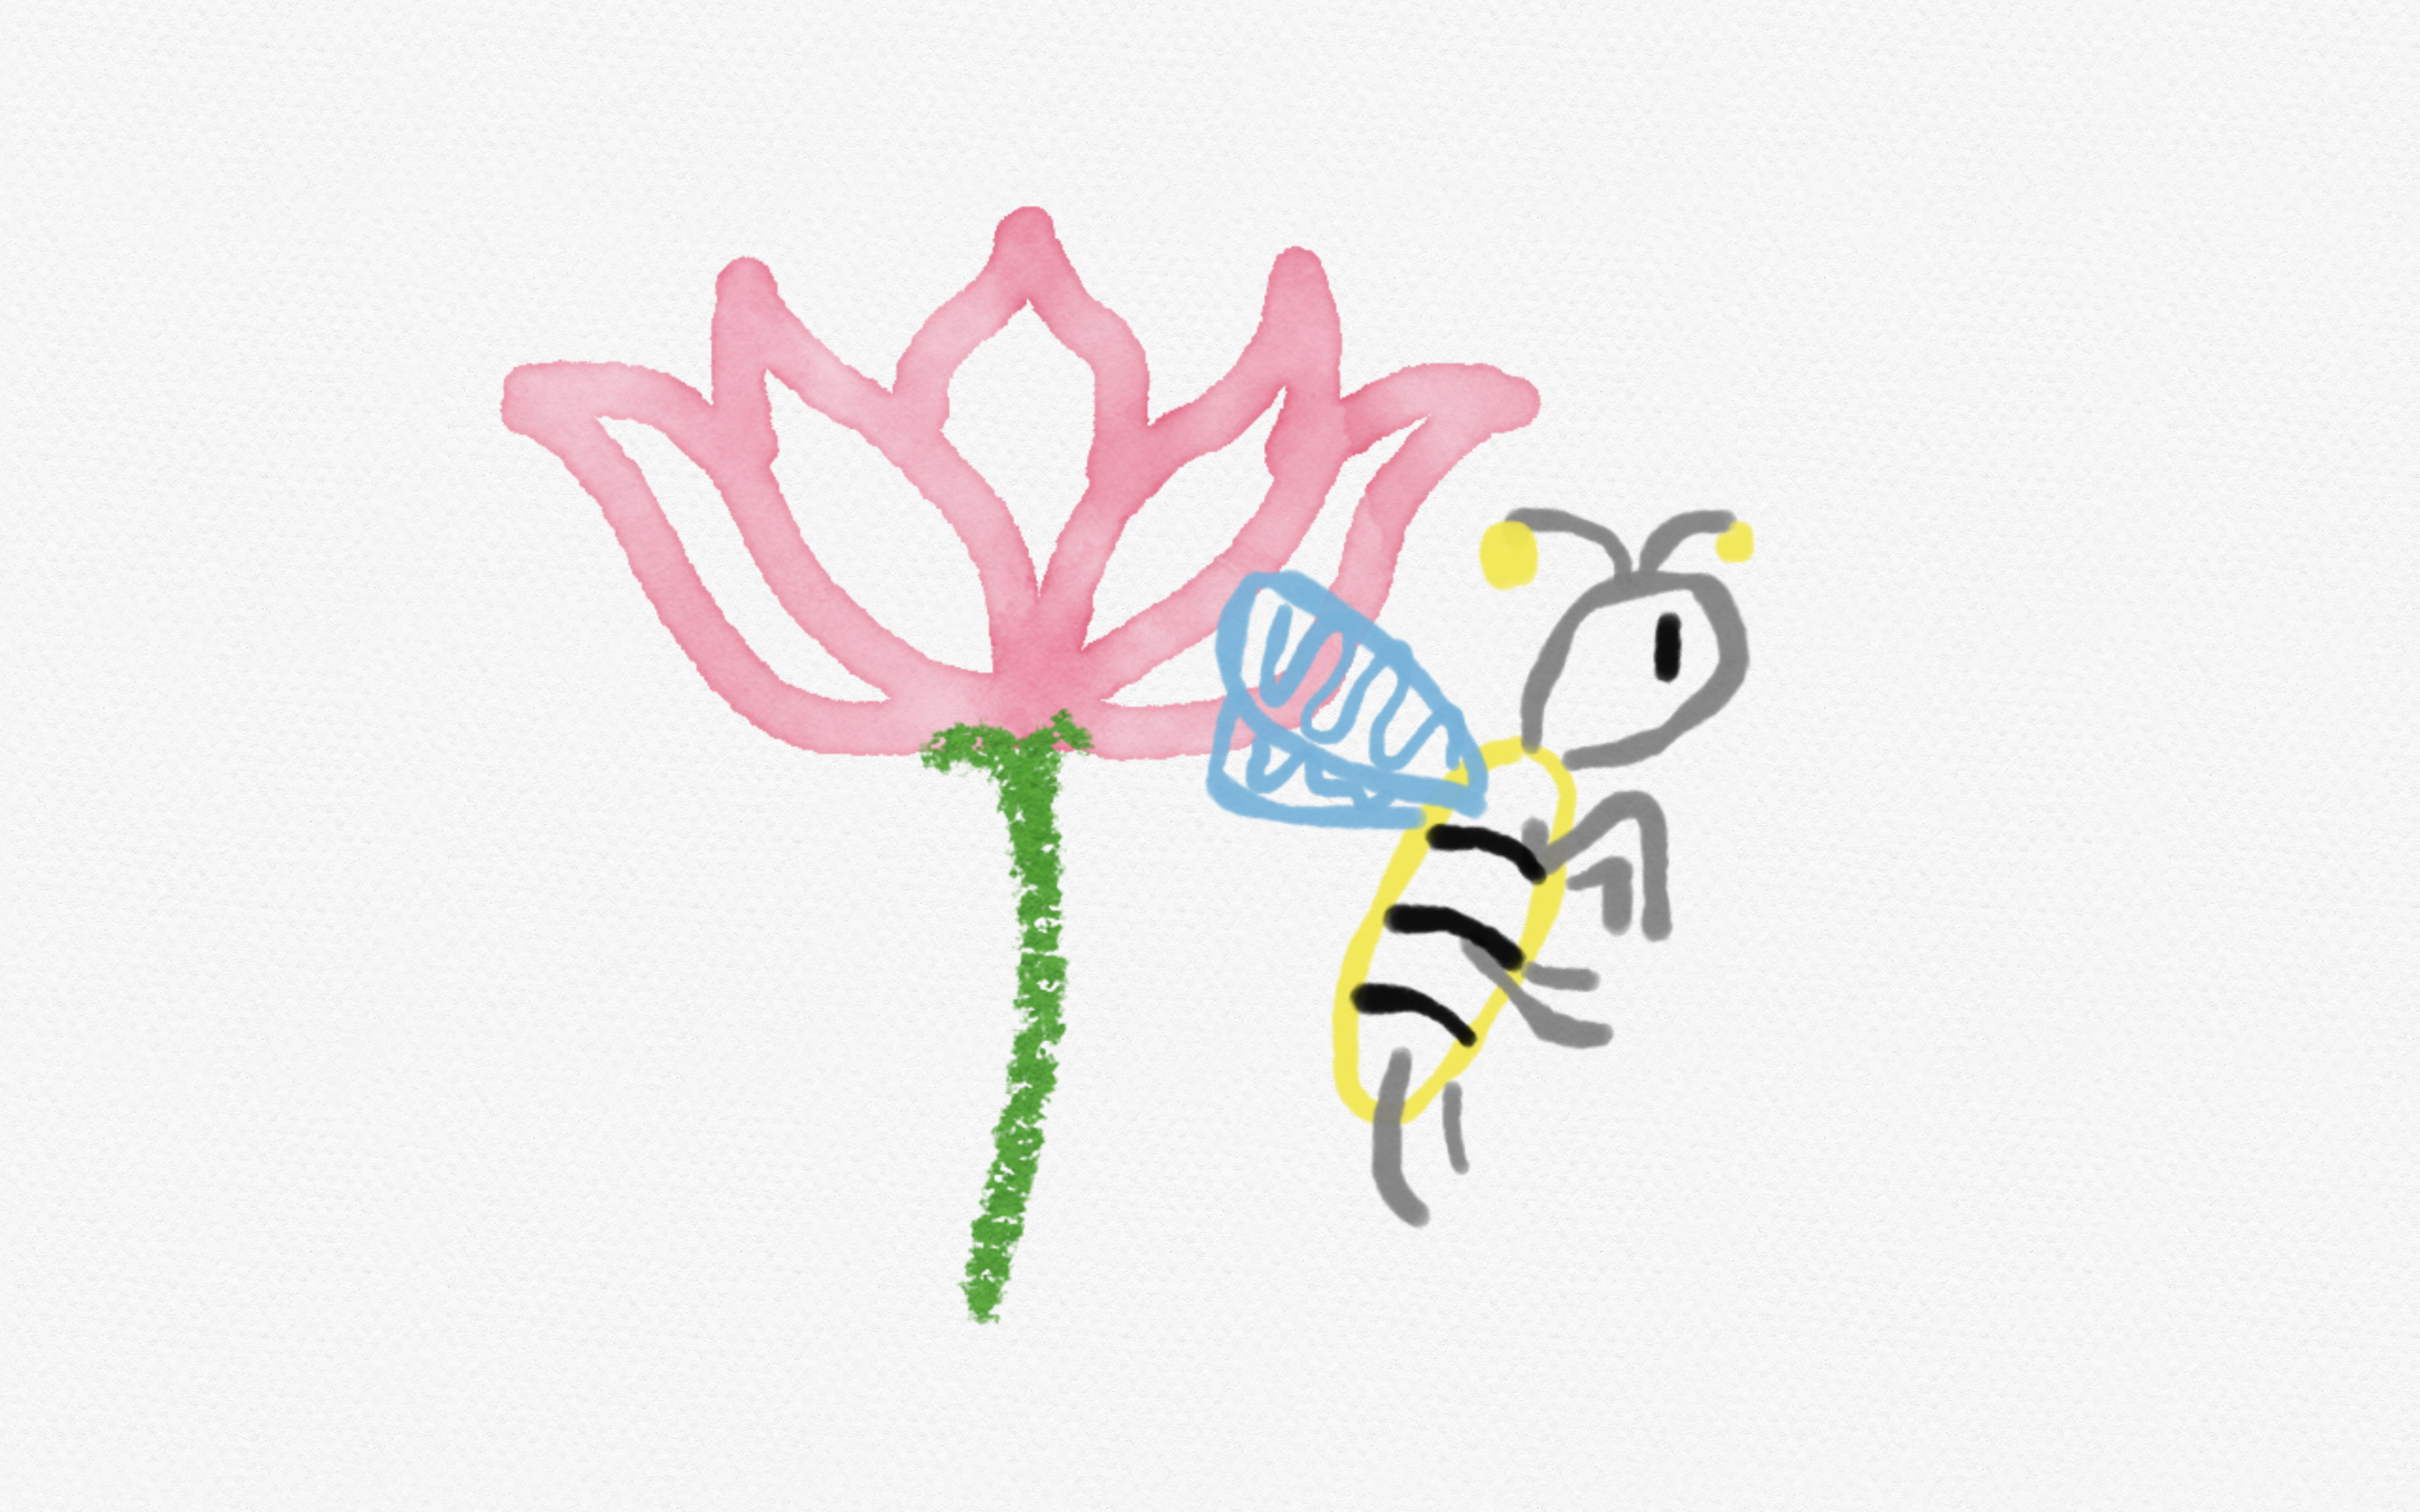
\includegraphics[width = 30em]{Logo}
\end{figure}
\newpage
\tableofcontents
\newpage

%----------------------------------------------------------------------Kapitel 1--------------------------------------------------------------------------------------------

\section{Einleitung}
Bei diesem Dokument handelt es sich um die Feinspezifikation unseres Bibliothekssystems. Es baut direkt auf dem vorangegangenen Entwurf auf und enthält einen noch genaueren Umriss der zu erstellenden Applikation.

%----------------------------------------------------------------------Kapitel 2--------------------------------------------------------------------------------------------

\section{Systemarchitektur}
\sectionauthor{Ivan Charviakou}



\subsection{Einführung}

Die vorgestellte Bibliotheksanwendung wird in Java mittels einer MVC-Architektur unter Verwendung eines 2-Schichten Modells realisiert. Dabei wird JSF als grundlegendes Web-Framework verwendet. Der Vorteil dieser Modellierung ist die Einfachheit der Implementierung und die Modularität der Persistenzschicht. Aufgrund der wenig umfangreichen Businesslogik bietet aber eine separate Schicht im Gegensatz zum 2-Schichten Modell bei deutlichem Mehraufwand kaum zusätzliche Modularität. \vspace{0.5em}

Genauer – Das Model besteht aus den folgenden Schichten:
\begin{itemize}
	\item \textbf{Logikschicht:} Die Aufgabe dieser Schicht ist es, die Benutzerinteraktion, die Navigation, und die hierzu erforderliche Funktionalitäten zu kapseln.
	\item \textbf{Persistenzschicht:} Da manche Funktionalitäten aus der Logik eine Datenpersistenz voraussetzen, befasst sich diese Schicht mit dem Speichern und Laden von Daten aus einem oder mehreren Quellen. 
		Sie bietet außerdem weitere persistenzbezogene Funktionalitäten an, die von beiden Schichten benötigt werden. 
\end{itemize}



\subsection{Architekturdiagramm}

Das folgende Diagramm stellt die MVC-Architektur mit den Beziehungen zwischen den einzelnen Komponenten anhand der gegebenen Applikation dar. Dabei folgt die Komponentenaufteilung der Paketstruktur der Applikation. Zudem entsprechen die Farben, die die Komponente im Diagramm besitzen, den Farben im nachfolgenden Klassendiagramm.

\begin{figure}[H]
	\centering
	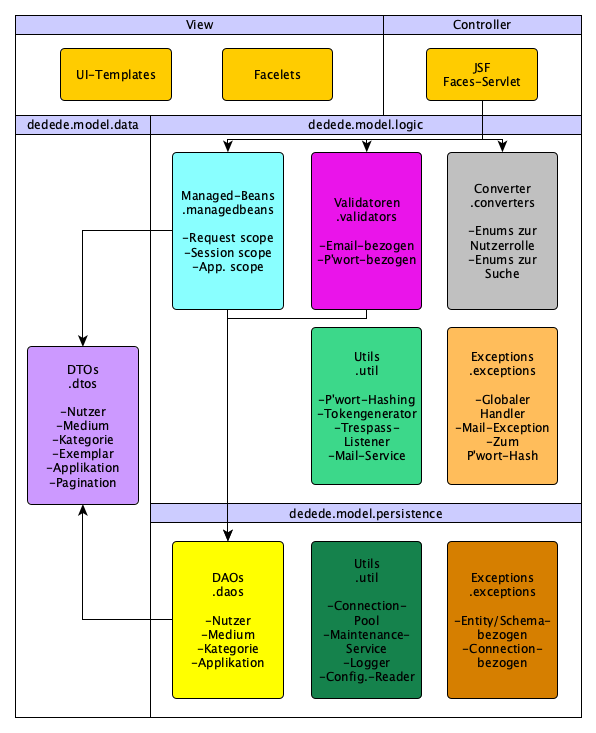
\includegraphics[width = 30em]{Modeldiagramm}
\end{figure}



\subsection{Paketstruktur}

Die verwendeten Java-Paketen werden im Folgenden aufgelistet und beschrieben:
\begin{itemize}
	\item \textbf{dedede.model.logic:} \hypertarget{Logikschicht}{Dieses Paket} bildet die gesamte Funktionalität der Logikschicht ab.
		\begin{itemize}
			\item \textbf{dedede.model.logic.managedbeans:} Dieses Paket enthält alle von der JSF-Applikation verwendeten Managed-Beans.
				Das sind unter anderem Backing-Beans, die von den Facelets referenziert werden, und jegliche Scoped-Beans, die diesen Backing-Beans zusätzliche Funktionalität bieten.
			\item \textbf{dedede.model.logic.validators:} Dieses Paket enthält alle von der JSF-Applikation für die Überprüfung der Benutzereingabe verwendeten Validatoren.
			\item \textbf{dedede.model.logic.converters:} Dieses Paket enthält alle von der JSF-Applikation verwendeten Converters.
			\item \textbf{dedede.model.logic.exceptions:} Dieses Paket definiert alle applikations-spezifische Exceptions, die von den Klassen aus der Logikschicht geworfen werden.
				Insbesondere sind das checked und unchecked Exceptions, die nur in der Logikschicht eine kontextuelle Bedeutung tragen.
			\item \textbf{dedede.model.logic.util:} Dieses Paket kapselt alle Funktionalitäten, von der die Funktionsweise der Logikschicht abhängt, aber auch über die direkte Benutzerinteraktion hinausgehen.
				Das sind unter andrem die E-Mail-Versendungsfunktionalität und die SystemEventListener-Implementierung, die für den Logikschicht-gesteuerten Systemstart und -stopp zuständig ist.
		\end{itemize}
	\item \textbf{dedede.model.persistence:} \hypertarget{DAOs}{Dieses Paket} bildet die gesamte Funktionalität der Persistenzschicht ab.
		\begin{itemize}
			\item \textbf{dedede.model.persistence.daos:} Dieses Paket enthält alle von der Applikation verwendeten Datenzugriffsobjekten (DAOs).
			\item \textbf{dedede.model.persistence.exceptions:} Dieses Paket definiert alle applikations-spezifische Exceptions, die von den Klassen aus der Persistenzschicht geworfen werden.
				Insbesondere sind das checked und unchecked Exceptions, die nur in der Persistenzschicht eine kontextuelle Bedeutung tragen.
			\item \textbf{dedede.model.persistence.util:} Dieses Paket kapselt alle Funktionalitäten, von der die Funktionsweise der Persistenzschicht abhängt.
				Dazu zählen unter anderem das Connection-Pool, das für die Datenbankverbindung notwendig ist, und der Wartungsthread, der die Integrität und Gültigkeit der persistierten Daten überwacht.
		\end{itemize}
	\item \textbf{dedede.model.data:} Dieses Paket stellt dem Applikationsmodell schichtenübergreifende Datenkonstruktionen bereit.
		\begin{itemize}
			\item \textbf{dedede.model.data.dtos:} Dieses Paket enthält alle von der Applikation verwendeten Datentransferobjekten (DTOs).
		\end{itemize}
\end{itemize}


\subsection{Design-Patterns}

\paragraph{Dependency-Injection:} % CDI
In JSF sorgt dieses Pattern dafür, dass eine Managed-Bean-Instanz einer Klasse automatisch bei der Instanziierung zur Verfügung gestellt wird. Dies unterscheidet sich von dem einfachen Anliegen eines Objekts dadurch, dass ein Managed-Bean mit einem größeren, Request-übergreifenden Scope wiederverwendet werden kann. In der gegebenen Anwendung wird dieses Pattern verwendet, um mit Hilfe von Scoped-Beans unter anderem den Applikations- und Session-Zustand zu modellieren. Als Beispiel wird in dem Session-Bean die Rolle eines Nutzers gespeichert, die bei der Nutzeranmeldung gesetzt wird. Durch Dependency-Injection bekommt das Backing-Bean der Medienansicht Zugriff auf diese Rolle, um Rollen-spezifische Funktionalitäten des Facelets anzuzeigen.

\paragraph{Factory-Pattern:}
Dieses Pattern erlaubt es, Objekte unabhängig von einer bestimmten Implementierung oder Einstellung zu erzeugen. Somit kann eine Implementierung dynamisch gewählt und leichter angepasst werden.
Um einen globalen Exception-Handler in JSF zu definieren, muss man als Beispiel zuerst den vorgegebenen Exception-Handler-Factory erweitern und diesen in den JSF-Konfigurationen registrieren.
Dieses Konstrukt erlaubt es, eigene Fehlerbehandlungsprozeduren als Wrapper-Klassen zu definieren, aus denen bei der Konstruktion eines Exception-Handlers ausgewählt wird.
Die einzige Funktionalität, die der globale Exception-Handler in der gegebenen Anwendung umsetzt, ist die Weiterleitung des Nutzers nur auf eine Fehlerseite. Trotzdem lässt sich mithilfe dieses Patterns weitere Funktionalitäten definieren.

\paragraph{Singleton-Pattern:} % Config-reader and logger
Das Singleton-Pattern sorgt dafür, dass ein Objekt im Lebenszyklus der Applikation nur einmal instanziiert wird. Ein wichtiger Vorteil eines Singletons ist die einfache Koordination von bestimmten Operationen.
In der gegebenen Applikation ist das Connection-Pool als Singleton realisiert. Dadurch wird unter anderem ein koordiniertes Herunterfahren aller Connections im System ermöglicht.

\paragraph{Object-Queuing:}
\hypertarget{Pooling}{Dieses Pattern} dient dazu, die Erzeugung von bestimmten Objekten zu beschränken und diese durch Vergabe und Rückgabe wiederverwendbar zu machen. Dies wird häufig in Fällen eingesetzt, in denen die Erzeugung von den Objekten als aufwendig gilt.
Durch Anwendung dieses Patterns werden die Connections aus dem Connection-Pool in ihrer Anzahl beschränkt, anderen Komponenten zur Verfügung gestellt, und anschließend an den Pool zurückgegeben.

\paragraph{Converter:}
Ein JSF-Converter hat die Aufgabe, für Objekte eine String-Darstellung zu berechnen, und für eine String-Darstellung ein Objekt. Dies wird in JSF verwendet, um Objekte in der View besser darstellbar oder auswählbar zu machen.
Beispielsweise sind für sämtliche Auswahllisten, die intern als Enum-Typen kodiert werden, Converter nötig. So werden unter anderem Nutzerrollen und Attributtypen kodiert.

\paragraph{Validatoren:}
Das in JSF eingebaute Validatoren-Konstrukt dient als erster Schutz gegen fehlerhafte Nutzereingaben.
In einem Validator wird eine Eingabe aus der View auf Korrektheit geprüft und im Fehlerfall eine Validator-Exception geworfen, die in der View als Folge eine Fehlermeldung erzeugt.
Als Beispiel von einem Validator aus der gegebenen Applikation dient der E-Mail-Validator. Bevor das System bei einer Registrierung eine E-Mail akzeptiert, wird nämlich überprüft, ob sie zu einem regulären Ausdruck passt.

\paragraph{Data Transfer Objects:}
Dieses Konstrukt kapselt zusammenhängende Daten zu einer oder mehreren Entitäten mit Hilfe von Gettern und Settern. Dabei enthält eine DTO keine Logik und wird als POJO implementiert.
Zudem werden DTO-Instanzen durch alle Modelschichten durchgereicht und erfüllen in jeder Schicht einen eigenen Zweck.
In der Persistenzschicht werden DTOs an DAOs übergeben und verwendet, um persistente Entity-Instanzen im Datenbestand zu aktualisieren, erstellen, oder löschen. DAOs dürfen auch DTOs erzeugen und befüllen.
In der Logikschicht werden DTOs zum einen aus der Persistenzschicht geholt, um persistierte Daten in der View anzuzeigen. Zum anderen werden sie in der Logikschicht durch Post-Construct-Methoden erzeugt, um von der View befüllt zu werden.

\paragraph{Data Access Objects:} % Static utility classes
Ein DAO wird verwendet, um Daten zu einer oder mehreren Entitäten mit Hilfe eines DTOs aus dem persistenten Datenbestand zu laden, löschen, aktualisieren, oder einzufügen.
Dabei sind komplexere Methodenformulierungen möglich und die verwendete Art von Datenpersistenz bleibt für die Logikschicht transparent.
Die DAOs in der gegebenen Anwendung unterstützen Transaktionsmanagement dadurch, dass öffentliche DAO-Steuermethoden package-private Methoden von anderen DAOs aufrufen dürfen.
Da die Implementierung der DAOs auf SQL ausgerichtet ist, werden Connection-Objekte durch diese package-private Methoden übergeben. Folglich sind die DAOs als statische Klassen realisiert.

\paragraph{Observer-Pattern:} % Explain usage more specifically
Dieses Pattern trennt die Rolle eines Observers und die eines Subjekts. Hierbei muss ein Observer dem Subjekt zugewiesen werden, um über Änderungen benachrichtigt zu werden.
Dadurch muss im Subjekt nicht fest-kodiert werden, wie viele Observer referenziert werden und welchen Typ sie besitzen.
In JSF liegt dieses Pattern einer Implementierung von einem Event- und Phasen-Listener zugrunde. Diese Listener werden nämlich als Observers verwendet, die auf bestimmte Events reagieren.

\paragraph{Phasen-Listener:} % TODO: Combine with Observer-pattern
Um unberechtigten Zugriff auf View-Ressourcen und Funktionalitäten zu vermeiden, werden mit Hilfe eines Phasen-Listeners die Nutzerberechtigungen geprüft.
Hierbei wird das Interface ‘PhaseListener‘ von JSF vorgegeben, deren Implementierungen lassen sich in der JSF-Konfiguration registrieren.
Falls die Nutzerberechtigungen für den angeforderten Zugriff nicht ausreichend sind, wird der Nutzer auf eine Fehlerseite weitergeleitet.
Der gleiche Mechanismus wird auch dazu verwendet, Tokens für eine Passwortrücksetzung oder E-Mail-Verifizierung zu registrieren oder entfernen.


\subsection{Fehlerbehandlung}

\paragraph{Logging:}
Ein wichtiger Aspekt der Fehlererkennung in der gegebenen Applikation ist das Logging-Framework. Durch einen Logger ist es möglich, den Ablauf der Anwendung und dabei entstehende Ereignisse in einer Log-Datei zu dokumentieren.
Der in der Applikation verwendete Logger definiert die Levels ‚SEVERE‘, ‚DETAILED‘ und ‚DEVELOPMENT‘ für Log-Einträge.
Da sowohl die Logik- als auch die Persistenzschicht den gleichen Logger verwendet, wird er in der gegebenen Applikation als schichtenübergreifendes Singleton implementiert.

\paragraph{Exception-Handling:}
Für jede Modellschicht werden eigene Checked-Exceptions definiert und verwendet. Die Behandlung oder ggf. das Weiterwerfen von diesen Exceptions geschieht in ‚try-catch‘-Blocken im aufrufenden Code.
Checked-Exceptions, die aus einer unteren Schicht stammen, können ebenfalls in ‚try-catch‘-Blocken in der oberen Schicht gefangen werden.
Um aber die Unabhängigkeit der Schichten zu unterstützen, wird stattdessen eine andere, schichten-spezifische Exception erzeugt und weitergeworfen.
Für die Behandlung von sämtlichen nicht-gefangenen Exceptions wird in der Applikation ein eigener globaler Exception-Handler vorgesehen, der den Nutzer auf eine Fehlerseite weiterleitet und die entsprechenden Details zu dieser Exception anzeigt.
Das sind unter anderem der Name, die Nachricht, und der Stack-Trace.



%----------------------------------------------------------------------Kapitel 3--------------------------------------------------------------------------------------------


%----------------------------------------------------------------------Kapitel 4--------------------------------------------------------------------------------------------


%----------------------------------------------------------------------Kapitel 5--------------------------------------------------------------------------------------------


%----------------------------------------------------------------------Kapitel 6--------------------------------------------------------------------------------------------


%----------------------------------------------------------------------Kapitel 7--------------------------------------------------------------------------------------------


%----------------------------------------------------------------------Kapitel 8--------------------------------------------------------------------------------------------


%----------------------------------------------------------------------Kapitel 9--------------------------------------------------------------------------------------------


\end{document}